% CASE STUDY
\section{Case Study}
The study fundamentally adheres to the requirements for providing a publicly provisioned blockchain infrastructure that delivers security, privacy, and efficiency at an enterprise-grade level. The Logos Blockchain is designed specifically for certain use cases rather than being a general-purpose blockchain. However, the security model that will be implemented in the Logos chain, and presented in detail in this study, especially in section 4 (Findings), can possibly be applicable to other blockchain frameworks. The findings primarily present the core principles and methodologies that can be adapted to enhance the security and performance of blockchain systems generally, before presenting the possible substrate-based solution. 

In this section (case study), the general description of the case is first outlined, where a theoretical model of a blockchain is defined in its "default" form. This means that at this stage, we define the blockchain with a base architecture that is generally considered as secure. In Section 2.2 (Requirements), the general security requirements for an enterprise-grade blockchain infrastructure are presented. This leads to Section 2.3 (Specifications), where this requirements are clearly specified and defined to create a comprehensive picture of what an enterprise-grade security model demands in terms of security and privacy.

\subsection{Definition}
For research purposes, we define a public blockchain based on the Substrate framework (many aspects can also be considered in a general context). This blockchain is a distributed digital ledger system that enables various participants to conduct transactions, execute smart contracts, and participate in the network's security and governance processes.


\subsection{Requirements}


\subsection{Specifications}

% FIGURE1
\begin{center}
	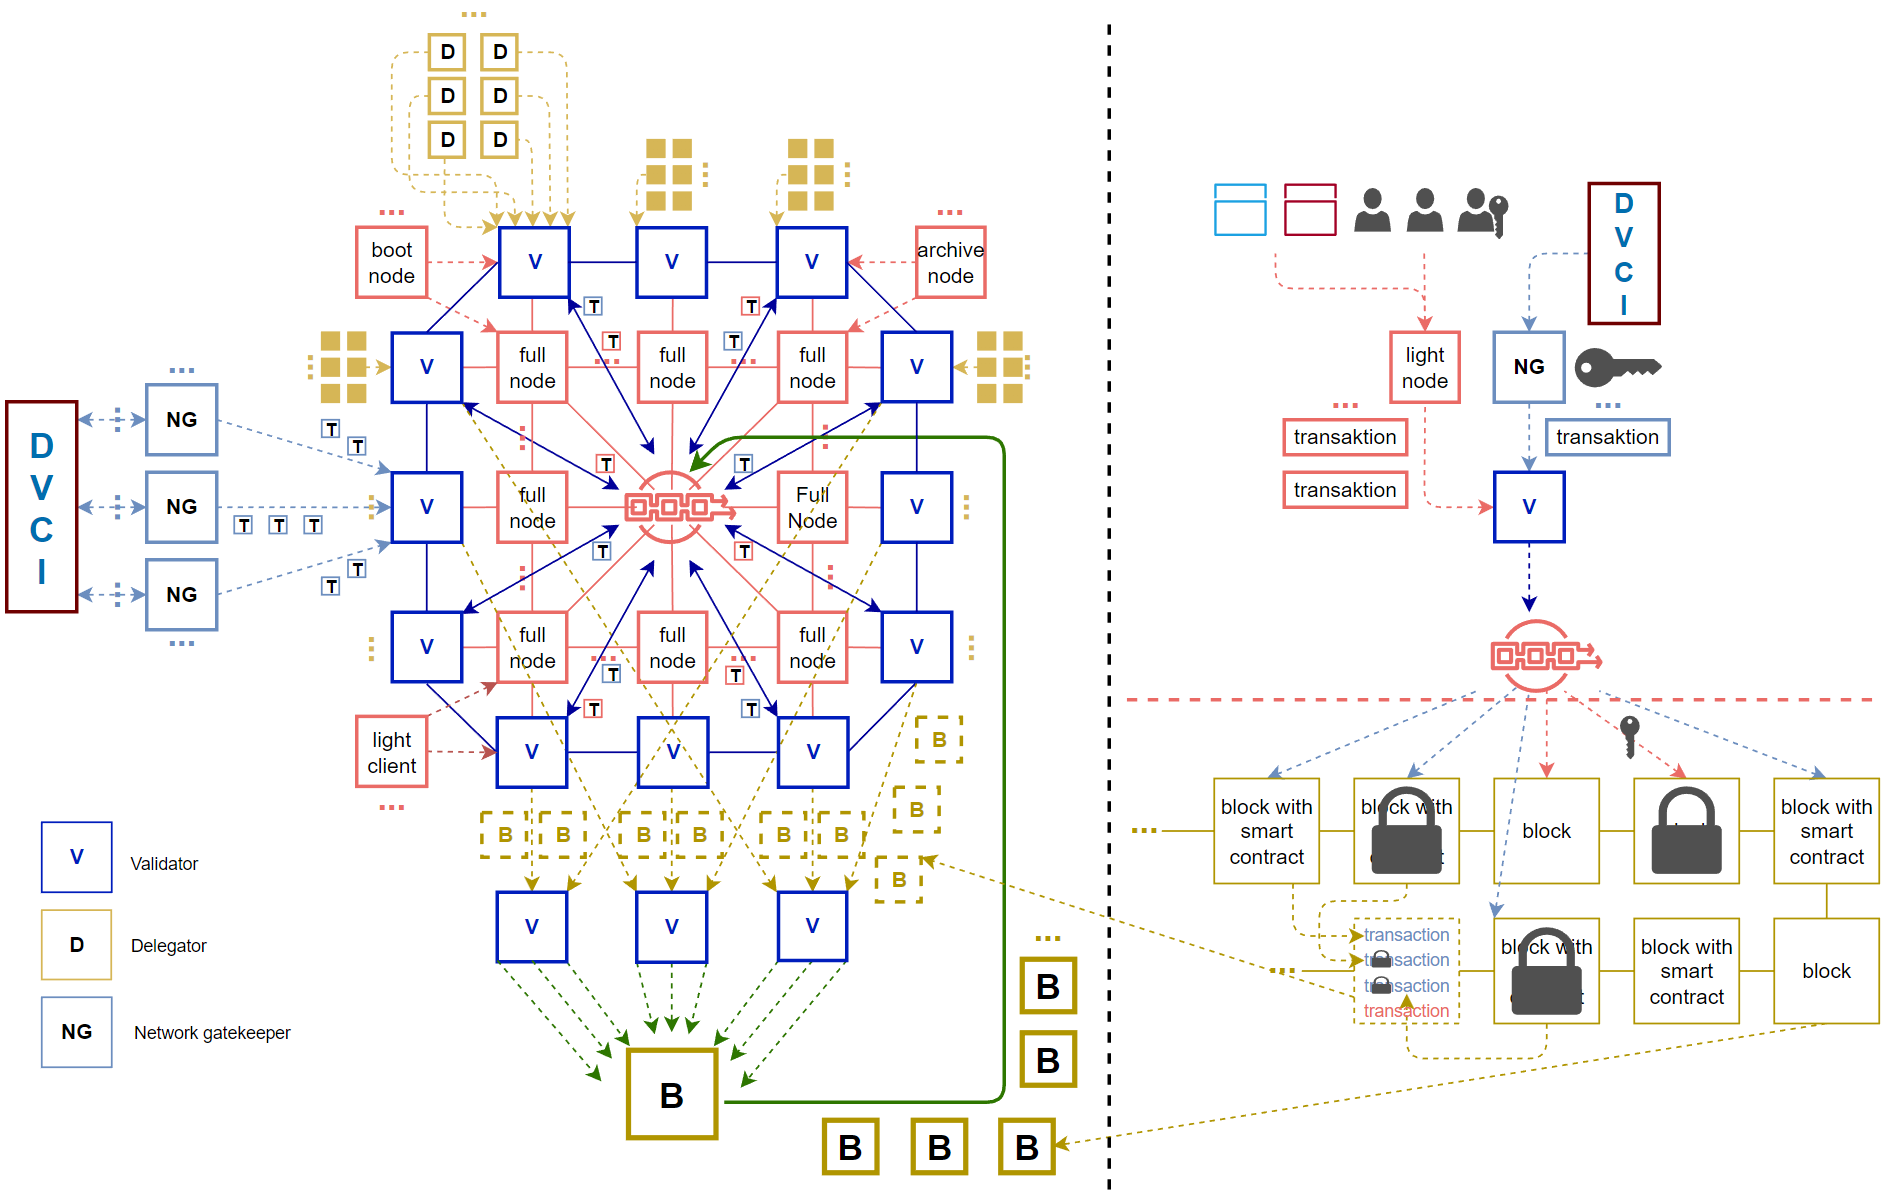
\includegraphics[height=10cm]{logos-chain}
\end{center}
\begin{center}
	Figure 1: 
\end{center}